	Na inicialização do projeto foi utilizado uma adaptação da técnica \textit{Inception Deck}, usada em metodologias ágeis, para a escrita do “termo” de abertura do projeto. Ela tem como objetivo estabelecer uma visão comum, entre todos os \textit{stakeholders}, sobre o que é o software, o que ele se dispõe a fazer. 

\subsection{Inception Deck - Projeto de Software}

	O \textit{Inception Deck} é composto por 10 seções que permitem alinhar as expectativas dos usuários quanto ao software que será desenvolvido. As seções são respectivamente: 1. Porque desenvolver o software; 2. Idealização do projeto; 3. Apresentação do Produto; 4. Definição do escopo do produto; 5. Usuários; 6. Arquitetura do produto; 7. Dificuldades do Projeto; 8. Tamanho do projeto; 9. Prioridades do projeto(tempo, custo, escopo) e 10. Definição do tempo e custo. Para se ajustar as necessidades do projeto as seções 8, 9 e 10 serão tratadas em apenas uma seção.


\textbf{Porque desenvolver o software}

	Esse seção elucida sobre as principais motivações que levaram ao desenvolvimento desse software.

	O software em desenvolvimento surgiu da necessidade de se obter uma  interface, na qual, o usuário pudesse interagir com uma bancada de teste de amortecedores. Suas principais funções consistem em configurar as informações necessárias para a execução dos testes, e a apresentação dos resultados em formato de relatório.


\textbf{Idealização e Escopo do projeto}

	Essa seção tem como objetivo caracterizar o software em desenvolvimento com o auxílio do \textit{framework} a seguir, e delimitar o escopo do produto, apresentando o que ele pretende fazer e o que ele não pretende.


	O software está sendo desenvolvido:
	\begin{itemize}
		\item \textbf{Para} Acadêmicos (Alunos e Professores) da Engenharia Automotiva
		\item \textbf{Que} precisam realizar testes em amortecedores de veículos leves
		\item \textbf{O} software em desenvolvimento
		\item \textbf{É} um aplicativo wep/app
		\item \textbf{Que} é responsável por fornecer os resultados do teste, em formato de relatório com gráficos específicos, após o mesmo ter sido configurado
		\item \textbf{Diferente de} soluções que não apresentam um resultado final em formato de relatório
		\item \textbf{Nosso produto} permite configurar vários tipos de testes de amortecedores, bem como, manter um histórico dos testes realizadas e amortecedores testados.
	\end{itemize}

	Escopo do produto:
	
	% Lembrar o povo de incluir essa biblioteca --->>>>>> \usepackage{booktabs}
	\begin{table}[!h]
		\centering
		\caption{Escopo do software em desenvolvimento}
		\label{escopo}
		\begin{tabular}{cc}
		\hline
		\rowcolor[HTML]{C0C0C0} 
		{\color[HTML]{000000} \textbf{Dentro do Escopo}} & {\color[HTML]{000000} \textbf{Fora do Escopo}} \\ \hline
		{\color[HTML]{000000} \begin{tabular}[c]{@{}c@{}}Fornecer uma interface entre o\\  usuário e a bancada\end{tabular}} & {\color[HTML]{000000} \begin{tabular}[c]{@{}c@{}}Fornecer comparação entre\\  os amortecedores\end{tabular}} \\ \hline
		{\color[HTML]{000000} \begin{tabular}[c]{@{}c@{}}Realizar a seleção e\\ configuração do teste\end{tabular}} & {\color[HTML]{000000} \begin{tabular}[c]{@{}c@{}}Realizar a simulação de um teste\\  apenas pelo software da bancada\end{tabular}} \\ \hline
		{\color[HTML]{000000} \begin{tabular}[c]{@{}c@{}}Apresentar os resultados do teste\\ num formato de relatório\end{tabular}} & {\color[HTML]{000000} } \\ \hline
		\end{tabular}
	\end{table}


\textbf{Usuários}

	Esse seção define toda comunidade possivelmente interessada no software, o que inclui, tanto os desenvolvedores, quanto acadêmicos, além de pessoas de outras áreas.

	\begin{figure}[h]
		\centering
		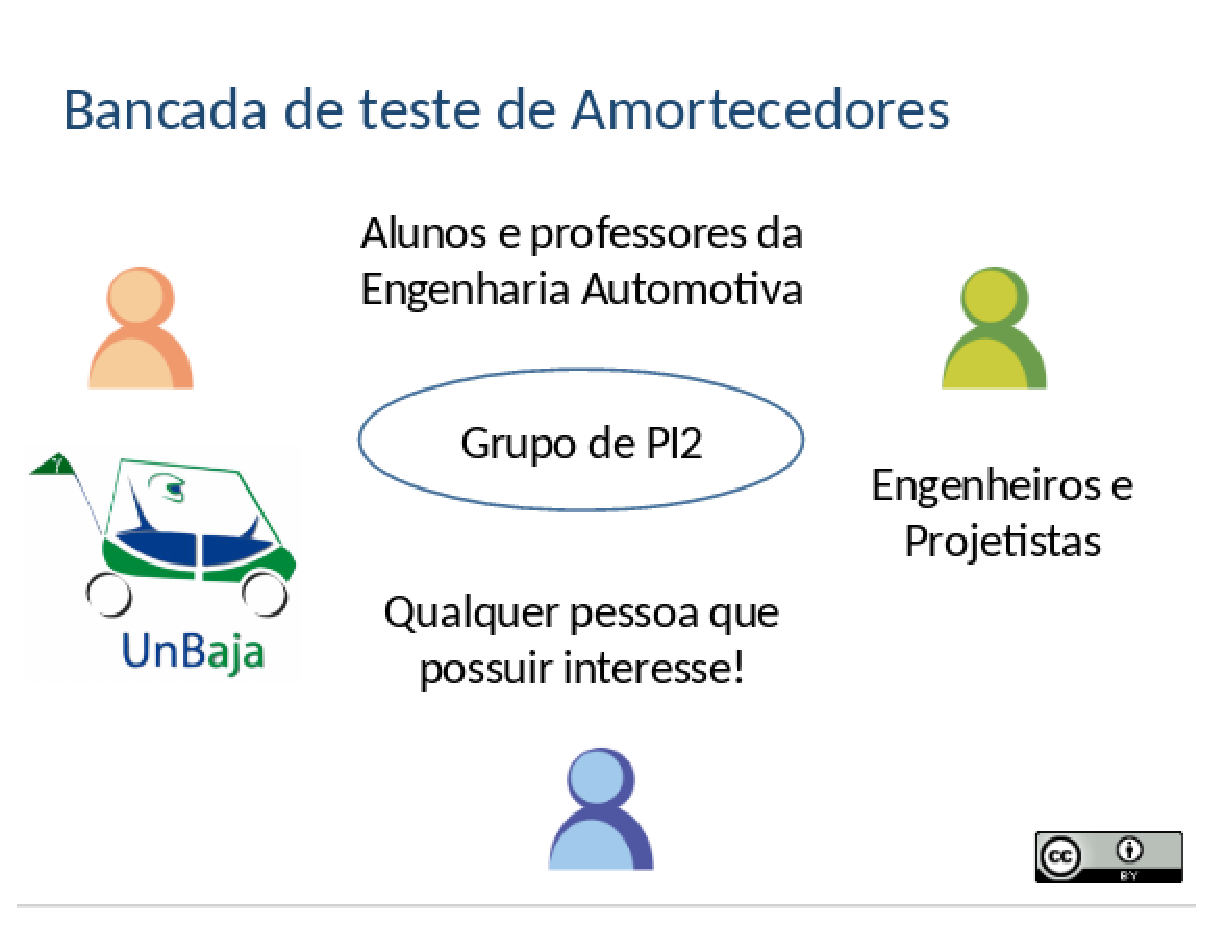
\includegraphics[width=0.8\textwidth]{resource/usuarios.eps}
		\caption{Comunidade de usuários do software}
		\label{img:usuarios}
	\end{figure}


\textbf{Arquitetura do produto}

	Essa seção é responsável por apresentar a arquitetura definida pelo time de desenvolvimento, bem como, descrever o suporte tecnológico.

	% TODO - atualizar
	A arquitetura de software será modelada em três camadas distintas, mas que estabelecem uma comunicação entre si. Esta estratégia foi adotada por permitir a modularização entre as camadas, pois apesar de uma camada necessitar da outra para o funcionamento total do bancada, será possível executar os testes de sistema separadamente em cada camada. Assim, os problemas encontrados em uma camada podem ser resolvidos facilmente sem necessariamente afetar as demais. A imagem \ref{arquiteturaSOFT} apresenta o diagrama da arquitetura estabelecida.

	\begin{figure}[h]
		\centering
		\includegraphics[width=1\textwidth]{arquiteturaSOFT}
		\caption{Arquitetura do Projeto de Software}
		\label{arquiteturaSOFT}
	\end{figure}

	O software será dividido em 3 camadas:
	Cliente;
	Processamento dos Dados e;
	Controlador da Bancada.

	A equipe de Engenharia de Software ficará responsável por implementar os módulos 1 e 2 e a equipe de Engenharia Eletrônica ficará responsável por implementar o módulo 3.

	\textbf{Modulo 1}

	O primeiro módulo, cliente, será responsável por estabelecer a comunicação do usuário com a bancada a fim de estabelecer um canal de comunicação para a entrada/saída de dados. Para isso, desenvolvera-se uma aplicação \textit{web-app} o qual será embarcada no microcontrolador e assim, ausenta a necessita do usuário final ter um aplicativo específico para interagir com o sistema, sendo necessário apenas um \textit{browser} a partir de um dispositivo que permita conexão via wi-fi. Este primeiro módulo será desenvolvido utilizando a linguagem Python v.3.4.3 utilizando \textit{framework} Django v.1.9. 

	Apesar do Django apresentar um arquitetura própria baseado no MVC (Model-View-Controller), o \textit{framework} permite a inserção de padrões de software sobre a medida do desenvolver conforme suas necessidades.

	\textbf{Modulo 2}

	O segundo módulo será responsável por estabelecer a comunicação com a base de dados e realizar o tratamento adequada dos dados oriundos dos sensores da bancada. Este tratamento está relacionado à forma como os dados são fornecidos a partir do microcontrolado, os quais serão disponibilizados pelo módulo três. Além disso, os dados que serão disponibilizados pelo módulo três estarão em formato CSV, isto é, os valores contido no arquivo serão separados por virgulas.

	A base de dados que será utilizada é o PostgreSQL por ser uma ferramenta de fácil utilização, escalável e gratuita. E o módulo será desenvolvido, em sua totalidade, em Python v.3.4.3.


	\textbf{Modulo 3}

	Já o terceiro módulo tem a responsabilidade de gerir o controle dos dados de entrada e saída da bancada. Ou seja, ele é incumbido de receber e repassar as informações que chegam dos sensores e também acionar na bancada as informações fornecidas pelo software. Este módulo, especificamente, será desenvolvido pela equipe da engenharia eletrônica. Para este módulo a principal linguagem utilizada será o ANSI C.


	A imagem a seguir, \ref{img:modulos}, ilustra os relacionamentos das três camadas sobre uma perspectiva mais detalhada.

	\begin{figure}[h]
		\centering
		\includegraphics[width=0.8\textwidth]{resource/modulos.png}
		\caption{Diagrama representativo da arquitetura proposta}
		\label{img:modulos}
	\end{figure}

	O cliente, a partir de uma camada de mapeamento de URL para TEMPLATE, requisitará uma página web. A URL terá o papel de associar a página requisitada a uma VIEW que posteriormente montará a página web a partir dos objetos (modelos) provindos da camada MODEL e das validações geridas pela camada TEMPLATE. A camada VIEW fará a comunicação com o suporte ao microcontrolador que por sua vez, estabelece a comunicação com a base de dados PostgreSQL. A camada onde encontra-se o microcontrolador receberá os comandos de acionamento da bancada a partir do módulo de suporte e também encaminhará para este módulo os resultados coletados pelos sensores.

\textbf{Dificuldades do Projeto}

	A Tabela \ref{tab:risco} lista as dificuldades idenficadas em forma de risco e as ações necessárias para mitigá-las.

	\begin{table}[h]
	\centering
	\caption{Risco para o Desenvolvimento do Software}
	\label{tab:risco}
	\resizebox{\textwidth}{!}{%
	\begin{tabular}{@{}ll@{}}
	\toprule
	\multicolumn{1}{c}{\textbf{Riscos}}                                   & \multicolumn{1}{c}{\textbf{Ações}}                                                \\ \midrule
	\multicolumn{1}{|l|}{Equipe não evoluir no desenvolvimento do App}    & \multicolumn{1}{l|}{Replanejar o escopo e promover um número maior de pareamento} \\ \midrule
	\multicolumn{1}{|l|}{Algum membro sem experiência na tecnologia}      & \multicolumn{1}{l|}{Realizar dojo para alinhamento do conhecimento}               \\ \midrule
	\multicolumn{1}{|l|}{Dificuldade para realizar reuniões presenciais}  & \multicolumn{1}{l|}{Realizar reunião on-line via Hangouts}                        \\ \midrule
	\multicolumn{1}{|l|}{Mudança muito grande dos requisitos do sistemas} & \multicolumn{1}{l|}{Priorizar histórias de usuário e redefinir escopo}            \\ \midrule
	\multicolumn{1}{|l|}{Descontinuidade de alguma biblioteca importante} & \multicolumn{1}{l|}{Repriorizar as tecnologias}                                   \\ \bottomrule
	\end{tabular}%
	}
	\end{table}

\textbf{Roadmap} 
\label{subsec:roadmap}

	Essa seção apresenta uma visão das funcionalidades presentes no software e quando elas serão entregues.

	\begin{figure}[h]
		\centering
		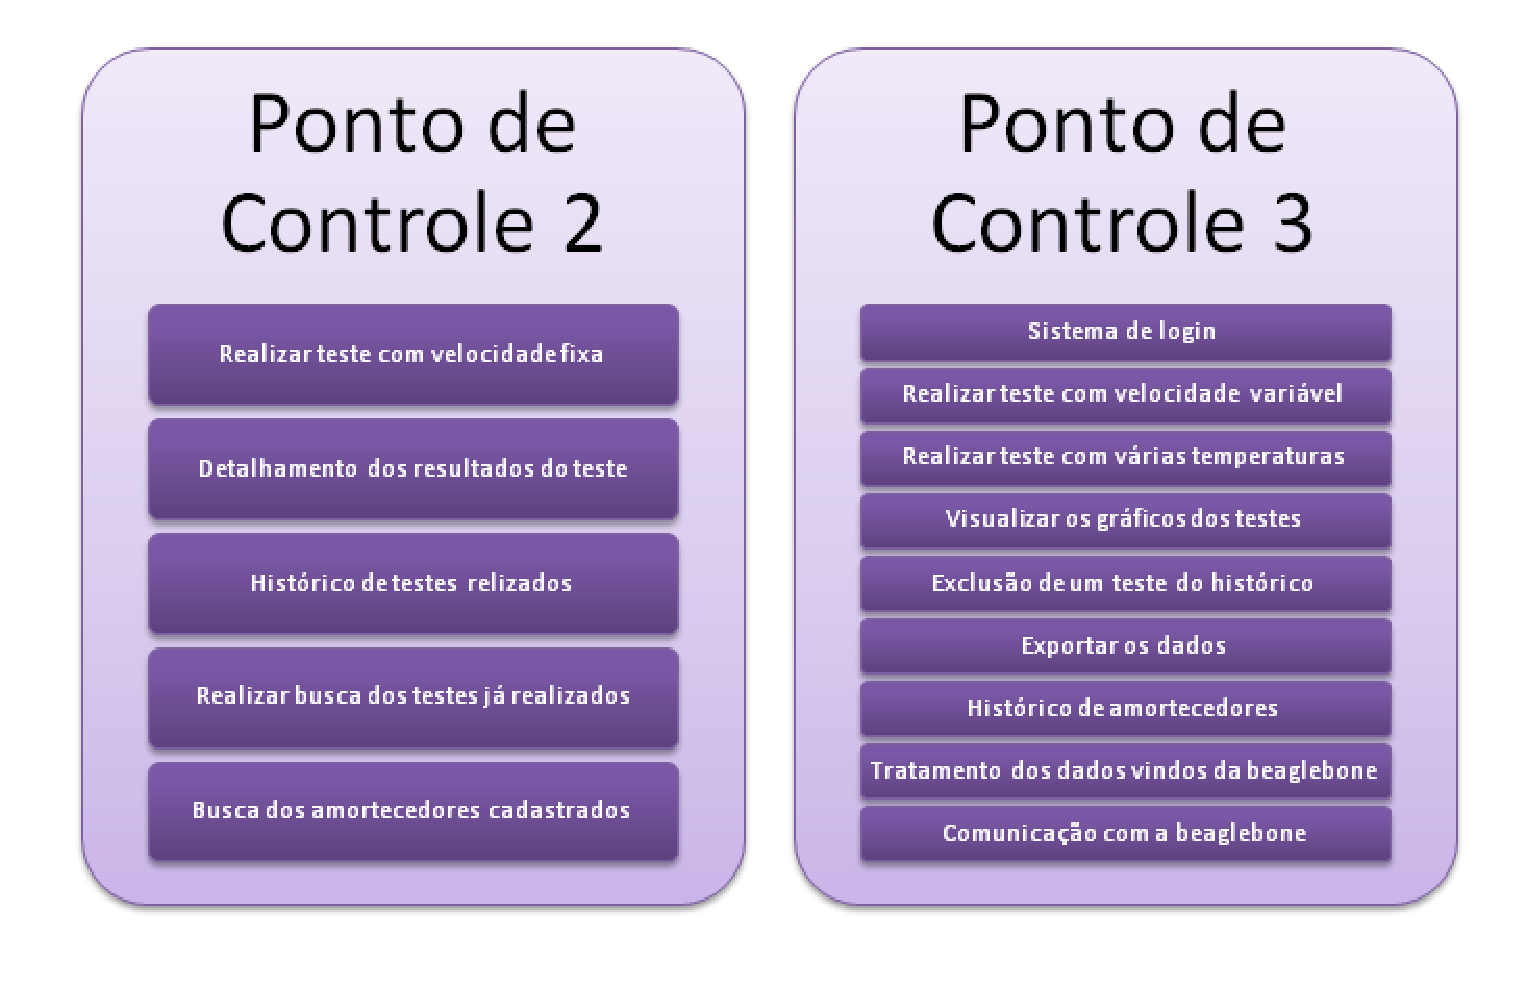
\includegraphics[width=1\textwidth]{resource/roadmap.eps}
		\caption{Funcionalidades previstas}
		\label{img:usuarios}
	\end{figure}


\subsection{Processo de Desenvolvimento}

	Com o objetivo de gerenciar o fluxo de desenvolvimento (implementação, teste unitário e teste de aceitação), adotou-se o uso do \textit{plugin} Zenhub. Este é instalado no \textit{browser}, ele altera a apresentação do site responsável por armazenar as versões do software, no caso desse trabalho o GitHub. O Zenhub cria uma \textit{dashboard}, Figura \ref{img:zenHub},  onde é possível separar as atividades em \textit{boards}. A utilização desse \textit{plugin} permite centralizar todas as informações referentes ao software.

	\begin{figure}[h]
		\centering
		\includegraphics[width=1\textwidth]{resource/zenHub.png}
		\caption{Ferramenta para Gestão de Requisitos - ZenHub}
		\label{img:zenHub}
	\end{figure}


\subsubsection{Gerenciamento dos Requisitos}

	Os requisitos sofrerão constantes atualizações, principalmente no que tange a definição dos dados a serem monitoradas durante o experimento da bancada. Para tanto, adotou-se a técnica de escrita de histórias de usuário segundo as metodologias ágeis, a fim, de aceitar as mudanças e manter um recorrente acompanhamento do software em relação a mecânica da bancada.

	Os requisitos não-funcionais acompanharam as historias de usuário mapeadas para testes de aceitação. Acredita-se que a maior parte destes requisitos está ligada a usabilidade e confiabilidade, principalmente em relação à acurácia dos cálculos e plotagens de gráficos.

	Para a elicitação das histórias de usuário foi realizado reuniões com a cliente principal, Larissa, graduanda em Engenharia Automotiva na UnB. As histórias foram armazenas em \textit{issues} no GiHub. \textit{Issue} é uma funcionalidade do GitHub que permite que os desenvolvedores possam armazenar as tarefas referentes ao desenvolvimento do projeto.

	Após a elicitação, os requisitos foram reunidos no \textit{backlog} do projeto, tabela \ref{USsoft}, sendo esses, priorizados e divididos em duas iterações. As iterações representam os marcos: Ponto de Controle 2 e Ponto de Controle 3. Os entregáveis de cada iteração são descritos no \textit{roadmap} do produto, apresentado na seção \ref{subsec:roadmap}.

	\newpage
	\begin{table}[]
		\centering
		\caption{Histórias de Usuário}
		\label{USsoft}
		\resizebox{\textwidth}{!}{%
		\begin{tabular}{ll}
		\hline
		\multicolumn{2}{c}{\textbf{Backlog do Produto}} \\ \hline
		\multicolumn{1}{c}{\textbf{ID}} & \multicolumn{1}{c}{\textbf{Descrição}} \\ \hline
		US1 & \begin{tabular}[c]{@{}l@{}}Como usuário, eu gostaria de ter um sistema de login para que apenas o\\ usuário logado possa realizar o teste.\end{tabular} \\ \hline
		US2 & Como administrador, eu gostaria de realizar um teste com velocidades fixas \\ \hline
		US3 & Como administrador, eu gostaria de realizar um teste com velocidades variáveis \\ \hline
		US4 & Como administrador, eu gostaria de realizar um teste com várias temperaturas \\ \hline
		US5 & \begin{tabular}[c]{@{}l@{}}Como administrador, eu quero visualizar os gráficos do teste para ter acesso\\ aos resultados\end{tabular} \\ \hline
		US6 & \begin{tabular}[c]{@{}l@{}}Como administrador, eu desejo excluir um teste realizado para manter o \\ histórico limpo de testes indesejados.\end{tabular} \\ \hline
		US7 & \begin{tabular}[c]{@{}l@{}}Como usuário, eu gostaria de ver os dados detalhados do teste para ter \\ acesso a todas as informações referentes ao teste\end{tabular} \\ \hline
		US8 & Como usuário, eu gostaria de exportar os dados do teste para que eu possa imprimi-los \\ \hline
		US9 & \begin{tabular}[c]{@{}l@{}}Como usuário, eu gostaria de visualizar o histórico dos testes para visualizar a lista dos \\ experimentos já realizados na bancada.\end{tabular} \\ \hline
		US10 & \begin{tabular}[c]{@{}l@{}}Como usuário, gostaria de realizar uma busca dos testes realizados na bancada para \\ que eu tenha acesso de forma rápida\end{tabular} \\ \hline
		US11 & \begin{tabular}[c]{@{}l@{}}Como usuário, eu gostaria de visualizar um histórico dos amortecedores para que eu\\  possa visualizar os amortecedores já cadastrados\end{tabular} \\ \hline
		US12 & \begin{tabular}[c]{@{}l@{}}Como usuário, gostaria de realizar uma busca dos amortecedores cadastrados\\ para que eu tenha acesso de forma rápida\end{tabular} \\ \hline
		\end{tabular}%
		}
	\end{table}

	Os testes de aceitação serão apresentados em uma seção posterior. Os demais testes, unitário e funcional, serão desenvolvimentos apenas na segunda iteração (último ponto de controle).


\subsubsection{Protótipos do Software}

	Os protótipos foram modelados com base no levantamento inicial dos requisitos de software. O sistema inicialmente foi estruturado em cinco telas as quais são ilustradas a seguir.
	
	\begin{figure}[h]
		\centering
		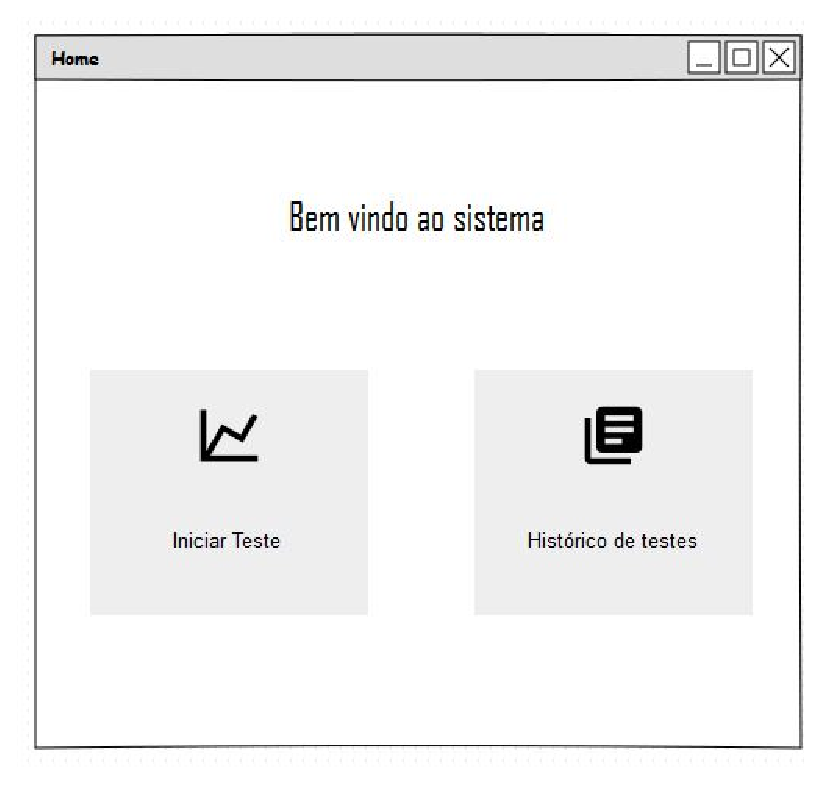
\includegraphics[width=0.6\textwidth]{resource/home.eps}
		\caption{Página inicial do sistema}
		\label{img:home}
	\end{figure}

	\begin{figure}[h]
		\centering
		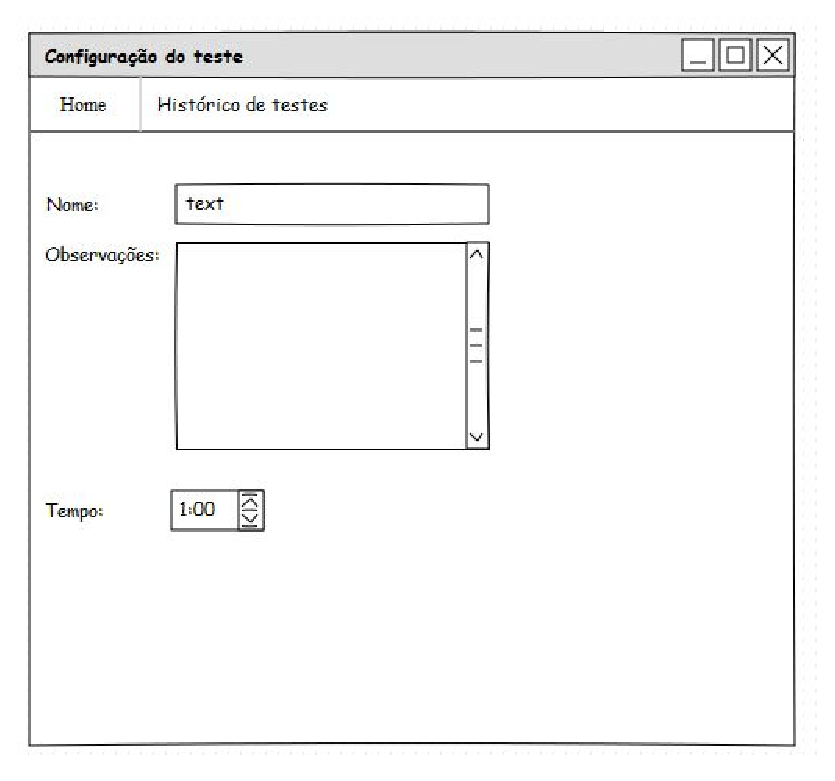
\includegraphics[width=0.6\textwidth]{resource/configteste.eps}
		\caption{Página de configuração do teste}
		\label{img:conf}
	\end{figure}

	
	\begin{figure}[h]
		\centering
		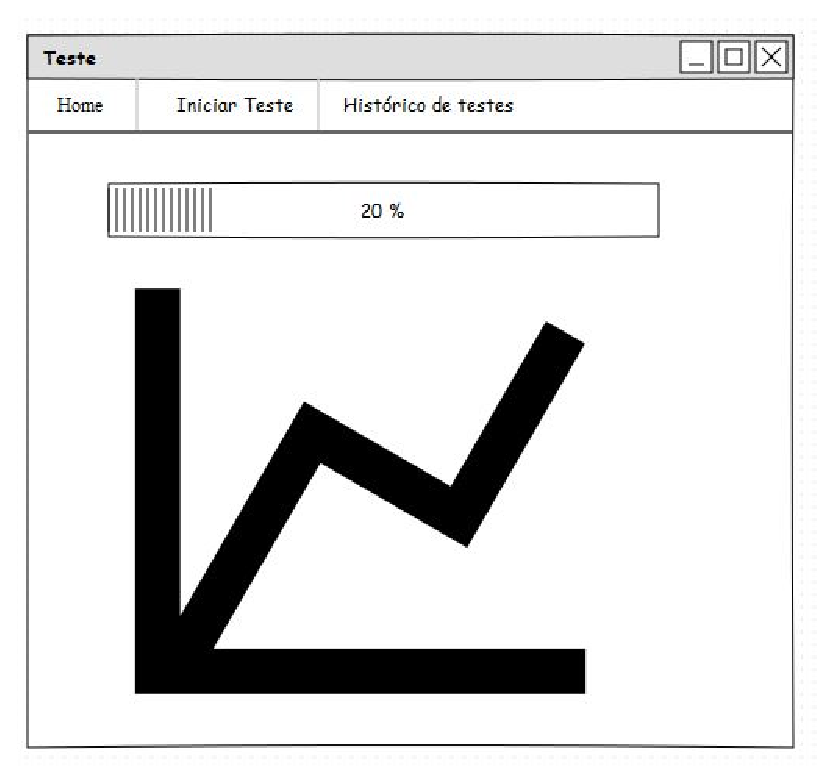
\includegraphics[width=0.6\textwidth]{resource/teste.eps}
		\caption{Realização do teste}
		\label{img:teste}
	\end{figure}


	\begin{figure}[h]
		\centering
		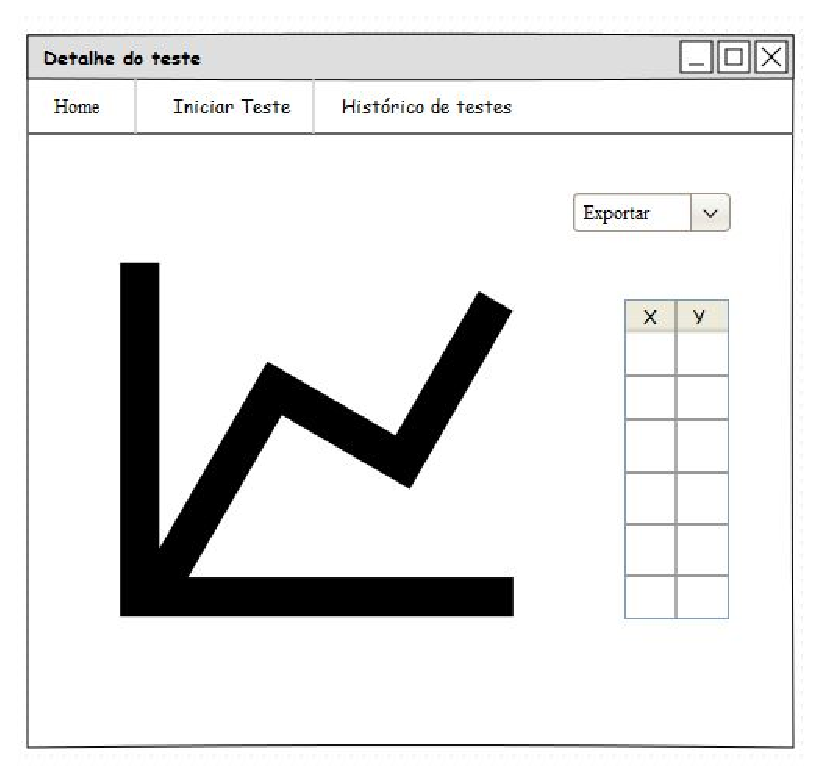
\includegraphics[width=0.6\textwidth]{resource/detalheteste.eps}
		\caption{Resultados dos testes}
		\label{img:detalhe}
	\end{figure}

	
	\begin{figure}[h]
		\centering
		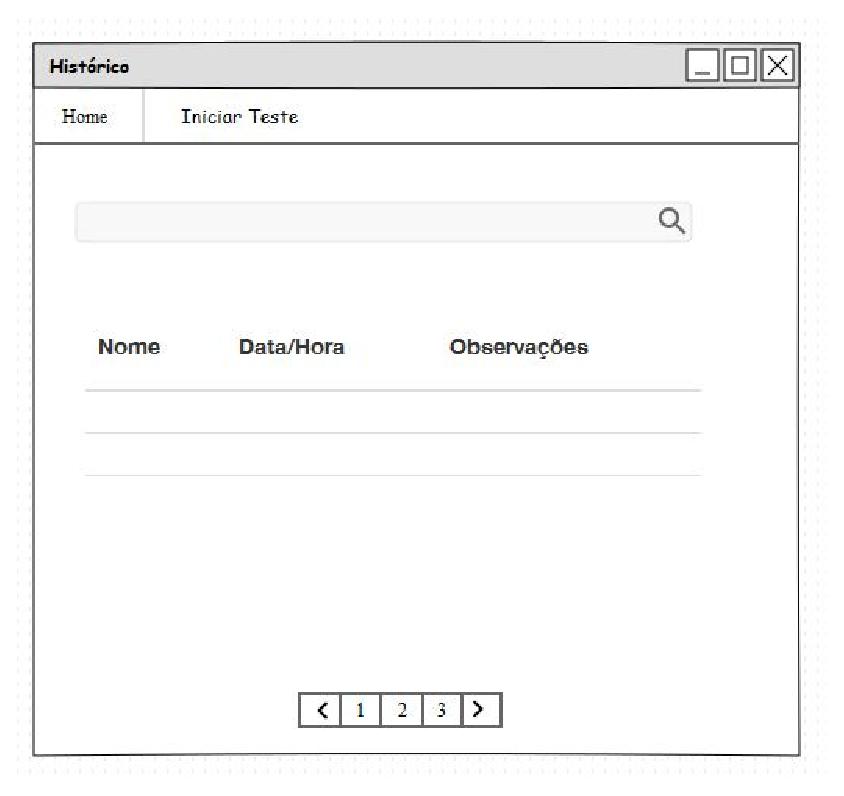
\includegraphics[width=0.6\textwidth]{resource/historico.eps}
		\caption{Histórico dos testes realizados}
		\label{img:historico}
	\end{figure}

\newpage
\newpage


\subsubsection{Suporte Tecnológico}
	A Tabela \ref{tab:tech} apresenta as tecnologias que auxiliaram o desenvolvimento do projeto.
	\newpage
	\begin{table}[h]
	\centering
	\caption{Tecnologias utilizadas}
	\label{tab:tech}
	\begin{tabular}{ccc}
	\hline
	\textbf{Ferramenta}              & \textbf{Versão}                   & \textbf{Função}                                                   \\ \hline
	\multicolumn{1}{|c|}{Git}        & \multicolumn{1}{c|}{mais recente} & \multicolumn{1}{c|}{Controle de versão}                           \\ \hline
	\multicolumn{1}{|c|}{GitHub}     & \multicolumn{1}{c|}{mais recente} & \multicolumn{1}{c|}{Armazenamento das versões}                    \\ \hline
	\multicolumn{1}{|c|}{ZenHub}     & \multicolumn{1}{c|}{mais recente} & \multicolumn{1}{c|}{Gerenciamento do desenvolvimento}             \\ \hline
	\multicolumn{1}{|c|}{Python}     & \multicolumn{1}{c|}{3.4.3}        & \multicolumn{1}{c|}{Linguaguem de desenvolvimento}                \\ \hline
	\multicolumn{1}{|c|}{Django}     & \multicolumn{1}{c|}{1.9.5}        & \multicolumn{1}{c|}{Framework para desenvolvimento Web em Python} \\ \hline
	\multicolumn{1}{|c|}{PostgreSQL} & \multicolumn{1}{c|}{9.4.7}        & \multicolumn{1}{c|}{Base de dados}                                \\ \hline
	\multicolumn{1}{|c|}{Highcharts} & \multicolumn{1}{c|}{4.2.4}        & \multicolumn{1}{c|}{Plotagem dos gráficos}                        \\ \hline
	\multicolumn{1}{|c|}{Bootstrap}  & \multicolumn{1}{c|}{3.3.6}        & \multicolumn{1}{c|}{Padronização dos templates das páginas web}   \\ \hline
	\multicolumn{1}{|c|}{Xhtml2pdf}  & \multicolumn{1}{c|}{0.1}          & \multicolumn{1}{c|}{Gerar PDF dos relatórios}                     \\ \hline
	\multicolumn{1}{|c|}{Psycopg2}   & \multicolumn{1}{c|}{2.5}          & \multicolumn{1}{c|}{Conexão com o banco de dados}                 \\ \hline
	\multicolumn{1}{|c|}{Debian}     & \multicolumn{1}{c|}{7}            & \multicolumn{1}{c|}{Sistema Operacional do microcontrolador}      \\ \hline
	\multicolumn{1}{|c|}{Pencil}     & \multicolumn{1}{c|}{mais recente} & \multicolumn{1}{c|}{Prototipação}                                 \\ \hline
	\end{tabular}
	\end{table}


% -------------------------------------------------------
\newpage
\newpage
\subsection{Desenvolvimento do Produto}
	
	Nesta seção apresenta-se algumas informações acerca do desenvolvimento do app.

	\subsubsection{Iterações}
		
		O projeto é composto por 6 iterações compreendido por 2 semanas. A tabela \ref{iteracoesSOFT} apresenta as iterações, suas respectivas datas de início e fim e metas para o grupo de Engenharia de Software.

		\begin{figure}[h]
			\centering
			\includegraphics[width=1\textwidth]{iteracoesSOFT}
			\caption{Metas das Iterações}
			\label{iteracoesSOFT}
		\end{figure}

		No momento, finaliza-se a iteração 4 realizando a reunião de retrospectiva levantando pontos fortes e fracos, estabelecendo assim ações de melhoria para a próxima iteração. E também dar-se inicio à iteração 5 com o principal objetivo finalizar o módulo módulo 1 (Aplicação Django) completamente, incluindo os testes de aceitação.

	\subsubsection{Repositório de Desenvolvimento}

		O repositório de desenvolvimento na ferramenta GitHub encontra-se disponível neste link:

		\href{https://github.com/ristovao/BancadaDeTesteParaAmortecedor}{https://github.com/ristovao/BancadaDeTesteParaAmortecedor}

	\subsubsection{Histórias de Usuário Desenvolvidas}

		A imagem \ref{andamentoSOFT} apresentada as histórias que já foram desenvolvidas e não desenvolvidas em um \% de conclusão.

		\newpage
		\begin{figure}[h]
			\centering
			\includegraphics[width=1.1\textwidth]{andamentoSOFT}
			\caption{(\%) de conclusão das Histórias de Usuário}
			\label{andamentoSOFT}
		\end{figure}

		Ainda deve ser desenvolvido os testes de aceitação para as histórias prontas. Os critérios de aceitação são apresentados nas imagens a seguir.

		\begin{figure}[h]
			\centering
			\includegraphics[width=1\textwidth]{CA01}
			\caption{Critérios de Aceitação das US - Parte 1}
			\label{CA01}
		\end{figure}

		\begin{figure}[h]
			\centering
			\includegraphics[width=1\textwidth]{CA02}
			\caption{Critérios de Aceitação das US - Parte 2}
			\label{CA02}
		\end{figure}

		\begin{figure}[h]
			\centering
			\includegraphics[width=1\textwidth]{CA03}
			\caption{Critérios de Aceitação das US - Parte 3}
			\label{CA03}
		\end{figure}

		\begin{figure}[h]
			\centering
			\includegraphics[width=1\textwidth]{CA04}
			\caption{Critérios de Aceitação das US - Parte 4}
			\label{CA04}
		\end{figure}

		\begin{figure}[h]
			\centering
			\includegraphics[width=1\textwidth]{CA05}
			\caption{Critérios de Aceitação das US - Parte 5}
			\label{CA05}
		\end{figure}

		\begin{figure}[h]
			\centering
			\includegraphics[width=1\textwidth]{CA06}
			\caption{Critérios de Aceitação das US - Parte 6}
			\label{CA06}
		\end{figure}

		\begin{figure}[h]
			\centering
			\includegraphics[width=1\textwidth]{CA07}
			\caption{Critérios de Aceitação das US - Parte 7}
			\label{CA01}
		\end{figure}





	




